\documentclass[letterpaper,11pt,oneside,reqno]{article}

%%%%%%%%%%%%%%%%%%%%%%%%%%%%%%%%%%%%%%%%%%%%%%%%%%%%%%%%%%%%

\usepackage[pdftex,backref=page,colorlinks=true,linkcolor=blue,citecolor=red]{hyperref}
\usepackage[alphabetic,nobysame]{amsrefs}

%%%%%%%%%%%%%%%%%%%%%%%%%%%%%%%%%%%%%%%%%%%%%%%%%%%%%%%%%%%%
%main packages
\usepackage{amsmath,amssymb,amsthm,amsfonts,mathtools}
\usepackage{graphicx,color}
\usepackage{upgreek}
\usepackage[mathscr]{euscript}

%equations
\allowdisplaybreaks
\numberwithin{equation}{section}

%tikz
\usepackage{tikz}
\usetikzlibrary{shapes,arrows,positioning,decorations.markings}

%conveniences
\usepackage{array}
\usepackage{adjustbox}
\usepackage{cleveref}
\usepackage{enumerate}
\usepackage{datetime}

%paper geometry
\usepackage[DIV=12]{typearea}

%%%%%%%%%%%%%%%%%%%%%%%%%%%%%%%%%%%%%%%%%%%%%%%%%%%%%%%%%%%%
%draft-specific
\synctex=1
% \usepackage{refcheck,comment}

%%%%%%%%%%%%%%%%%%%%%%%%%%%%%%%%%%%%%%%%%%%%%%%%%%%%%%%%%%%%
%this paper specific
\newcommand{\ssp}{\hspace{1pt}}

%%%%%%%%%%%%%%%%%%%%%%%%%%%%%%%%%%%%%%%%%%%%%%%%%%%%%%%%%%%%
\newtheorem{proposition}{Proposition}[section]
\newtheorem{lemma}[proposition]{Lemma}
\newtheorem{corollary}[proposition]{Corollary}
\newtheorem{theorem}[proposition]{Theorem}
%%%%%%%%%%%%%%%%%%%%%%%%%%%%%%%%%%%%%%%%%%%%%%%%%%%%%%%%%%%%
\theoremstyle{definition}
\newtheorem{definition}[proposition]{Definition}
\newtheorem{remark}[proposition]{Remark}
%%%%%%%%%%%%%%%%%%%%%%%%%%%%%%%%%%%%%%%%%%%%%%%%%%%%%%%%%%%%

\begin{document}
\title{Lectures on Random Matrices
(Spring 2025)
\\Lecture 12: Title TBD}


\date{Wednesday, April 2, 2025\footnote{\href{https://lpetrov.cc/rmt25/}{\texttt{Course webpage}}
$\bullet$ \href{https://lpetrov.cc/simulations/model/random-matrices/}{\texttt{Live simulations}}
$\bullet$ \href{https://lpetrov.cc/rmt25/rmt25-notes/rmt2025-l12.tex}{\texttt{TeX Source}}
$\bullet$
Updated at \currenttime, \today}}



\author{Leonid Petrov}


\maketitle
\tableofcontents


\section{Recap}

In our last lecture, we explored the asymptotics of Dyson Brownian Motion with an outlier. We specifically focused on the phase transition that occurs when a rank-1 perturbation is applied to a random matrix ensemble.

\subsection{Dyson Brownian Motion with Determinantal Structure}

We established that for $\beta=2$, the eigenvalues of the time-evolved process form a determinantal point process. The transition probability from an initial configuration $\mathbf{a} = (a_1 \geq \cdots \geq a_N)$ to a configuration $\mathbf{x} = (x_1 \geq \cdots \geq x_N)$ at time $t$ is given by:
\begin{equation*}
P(\lambda(t) = \mathbf{x} \mid \lambda(0) = \mathbf{a}) = N! \Big(\frac{1}{\sqrt{2\pi t}}\Big)^N \prod_{1\leq i<j\leq N}\frac{x_i - x_j}{a_i - a_j} \det\Big[\exp\Big(-\frac{(x_i - a_j)^2}{2t}\Big)\Big]_{i,j=1}^N
\end{equation*}

This determinantal structure enabled us to derive the correlation kernel:
\begin{equation}\label{eq:correlation-kernel}
K_t(x,y) = \frac{1}{(2\pi)^2 t} \int\int \exp\Big(\frac{w^2 - 2yw}{2t}\Big) \bigg/ \exp\Big(\frac{z^2 - 2xz}{2t}\Big) \prod_{i=1}^n \frac{w-a_i}{z-a_i} \frac{dw\,dz}{w-z}
\end{equation}
where the contours of integration are specified to maintain analytical properties.

\subsection{The BBP Phase Transition}

The central focus was the Baik-Ben Arous-Péché (BBP) phase transition that occurs with finite-rank perturbations of GUE matrices. For the rank-1 case, we analyzed:
\begin{equation*}
A + \sqrt{t}G, \quad \text{where } A = \text{diag}(a\sqrt{n},0,\ldots,0)
\end{equation*}

Through asymptotic analysis using steepest descent methods, we identified three distinct regimes:

\begin{enumerate}
\item \textbf{Airy regime} ($a < 1$): The largest eigenvalue follows the Tracy-Widom GUE distribution, just as in the unperturbed case. The spike is too weak to escape the bulk.

\item \textbf{Critical regime} ($a = 1$): A transitional behavior occurs when $a = 1 + An^{-1/3}$, leading to a deformed Airy kernel:
\begin{equation*}
\tilde{K}_{\text{Airy}}(\xi,\eta) = \frac{1}{(2\pi i)^2}\iint \frac{\exp\left\{\frac{W^3}{3}-\xi W-\frac{Z^3}{3}+\eta Z\right\}}{W-Z} \frac{W-A}{Z-A} dW\,dZ
\end{equation*}

\item \textbf{Gaussian regime} ($a > 1$): The largest eigenvalue separates from the bulk, becoming an "outlier" centered at $a + 1/a$. Its fluctuations follow a Gaussian distribution rather than the Tracy-Widom law.
\end{enumerate}


\subsection{Remark: Corners process with outliers}

One can also perturb the corners process structure, and get
correlation kernels similar to \eqref{eq:correlation-kernel} 
which we had for the Dyson Brownian Motion.
The perturbed corners process is
considered in \cite{Ferrari2014PerturbedGUE},
see also the earlier work \cite{Metcalfe2011GT}
for the corners process of $UDU^\dagger$, where $D$ is arbitrary and
$U$ is Haar-distributed. Both the kernels
for the Dyson Brownian Motion and the corners process
with outliers can be obtained from the formula of
\cite{Metcalfe2011GT}.
See \Cref{fig:outlier-evolution} for an illustration of the corners process with an outlier
in two cases, when the basis for the outlier is rotated or not
(the rotation does not affect the top level eigenvalue distribution,
but has a significant effect on the whole corners process).




\begin{figure}[]
	\centering
	\begin{tabular}{cc}
		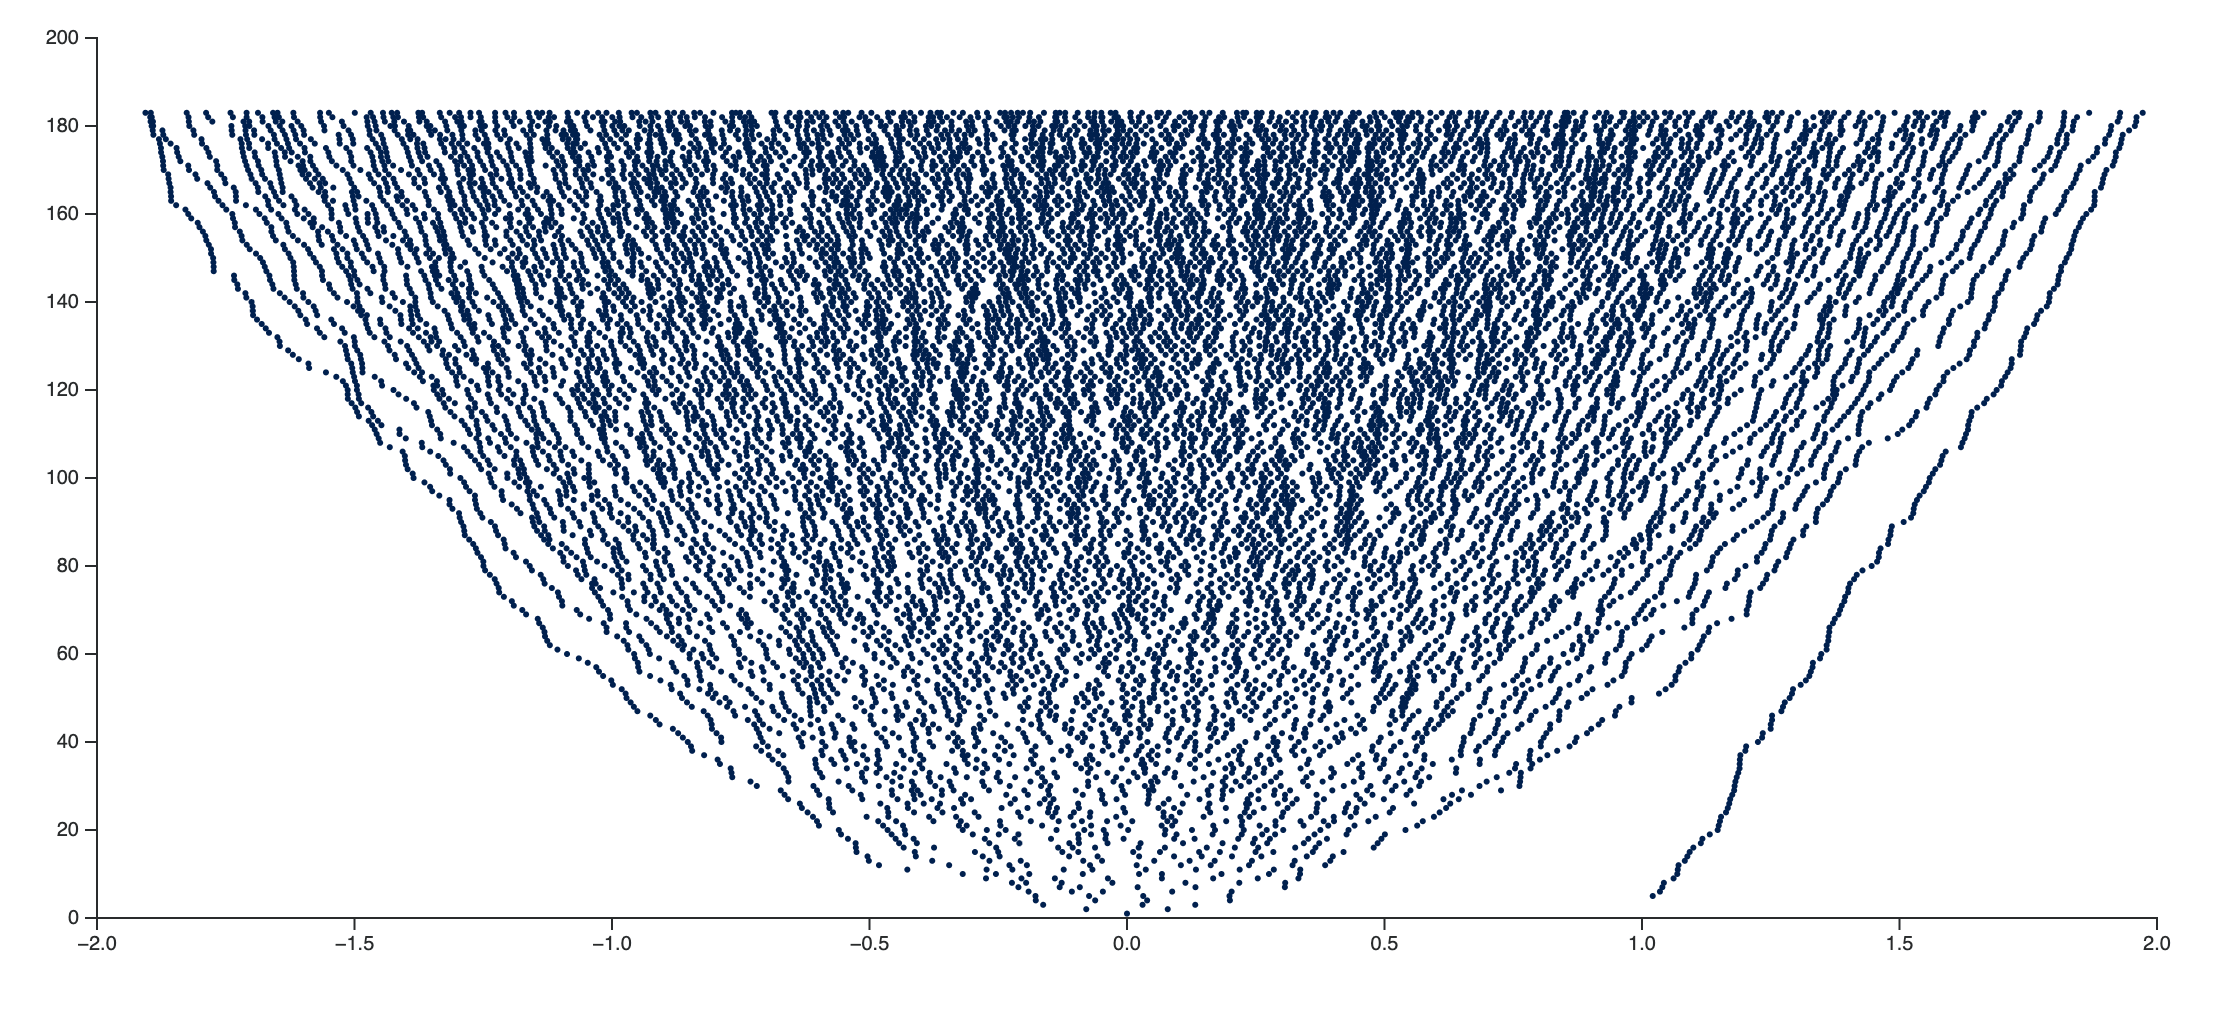
\includegraphics[width=0.45\textwidth]{pictures/outlier.png} &
		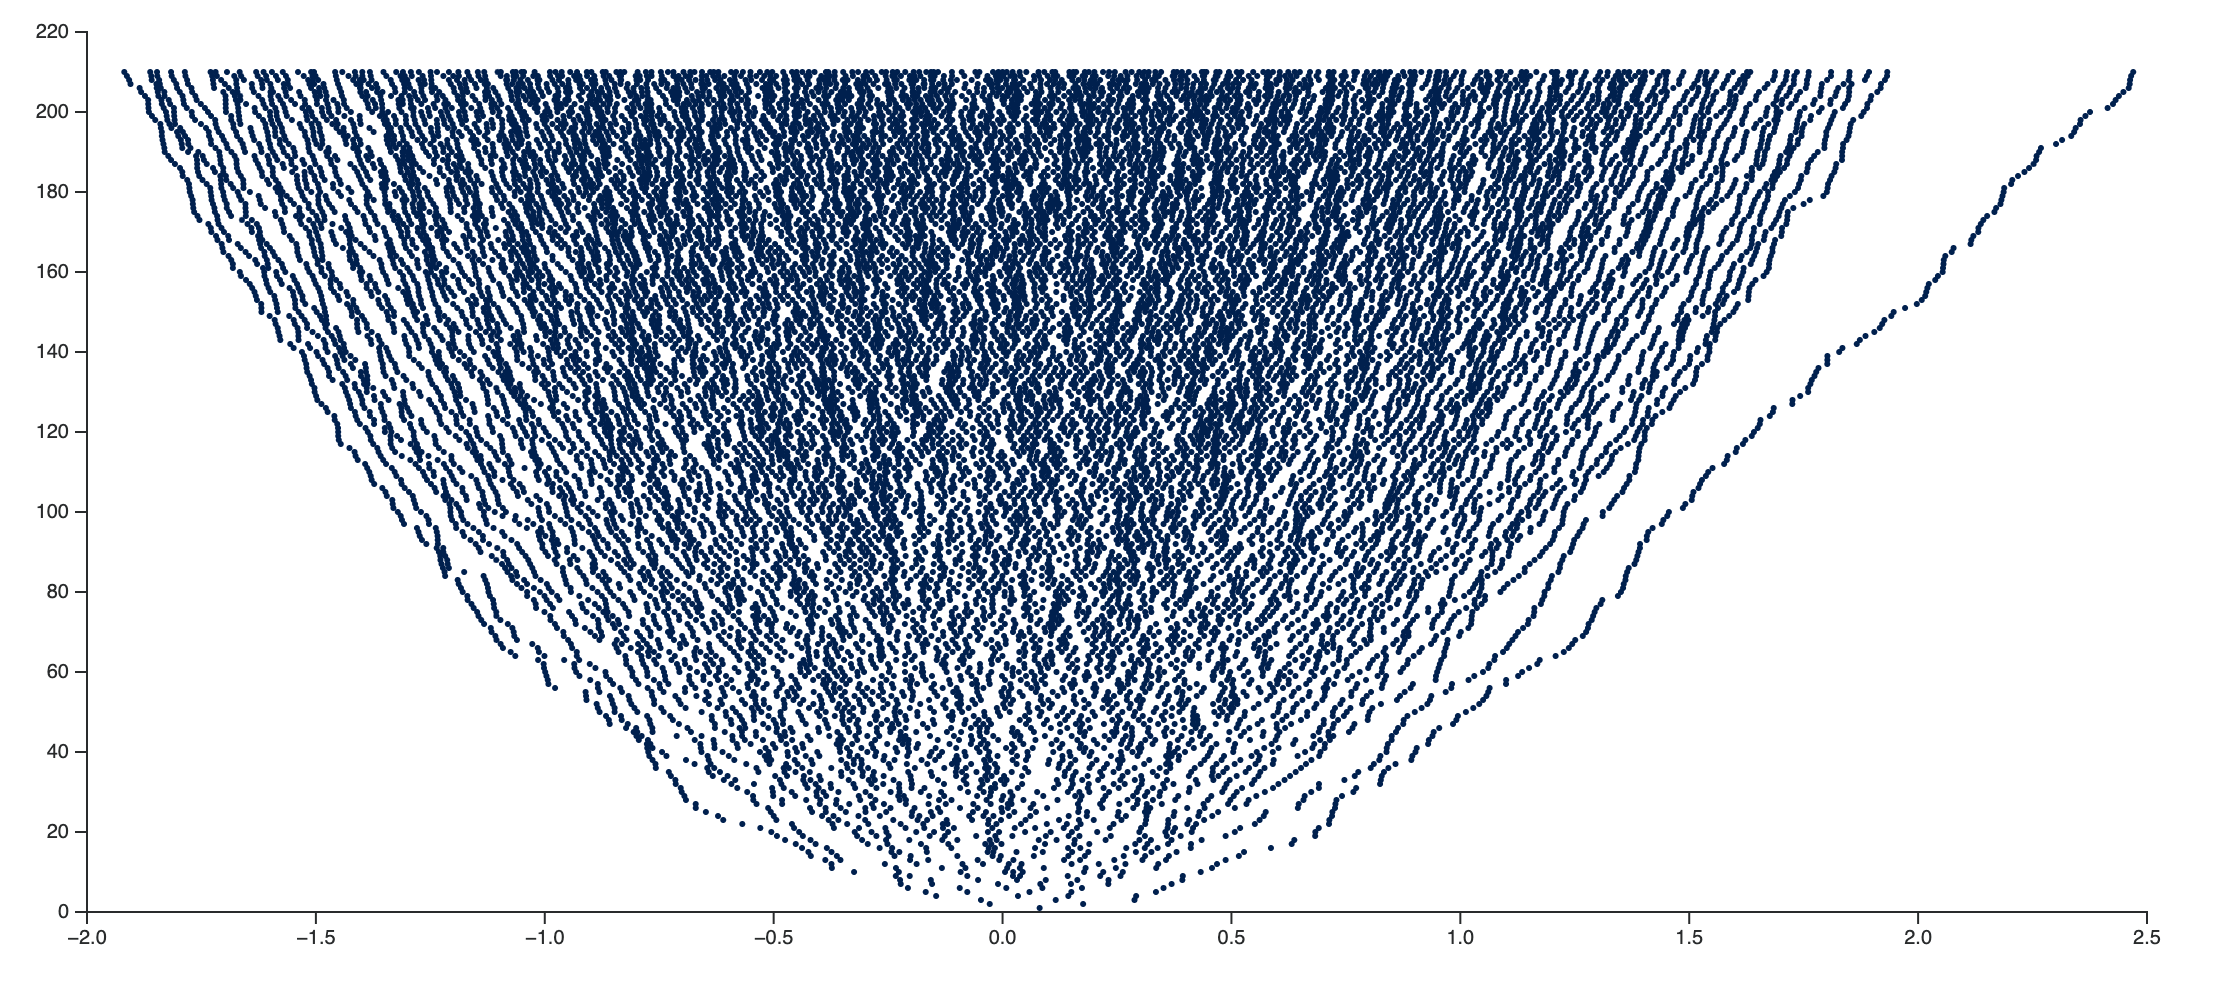
\includegraphics[width=0.45\textwidth]{pictures/rotated_outlier.png}
	\end{tabular}
	\caption{Two versions of the corners process with an outlier.
	Left: Corners process of $G+D$, where $D$ is a rank-1 critical perturbation with eigenvalue
	$1$. Right: Corners process of $G+UDU^\dagger$, where
	$U\in U(n)$ is a Haar-distributed unitary matrix and $D$
	is a rank-1 supercritical perturbation with eigenvalue $2$
	(the eigenvalue $1$ is not visible in the rotated system).
	In both pictures, $n\approx 200$. See
	\url{https://lpetrov.cc/simulations/2025-03-27-orthogonal-corners-outliers/}
	for an interactive simulation.}
	\label{fig:outlier-evolution}
\end{figure}


\section{A window into universality: Airy line ensemble}

The edge scaling limit of Dyson Brownian Motion is a universal object for $\beta=2$ models and determinantal structures (and far beyond); which includes the GUE Tracy-Widom distribution as a marginal. This is also intimately related to the KPZ universality class, which we will touch upon in the next few lectures.
GUE formulas
provide us with a powerful lens through which to examine these universality phenomena. In this section, we discuss the limiting behavior of Dyson Brownian Motion near the spectral edge, highlighting two of its fundamental properties: Brownian Gibbs property and characterization.

\begin{theorem}[Edge scaling limit to Airy line ensemble]
	Consider an $N\times N$ GUE (Gaussian Unitary Ensemble) Dyson Brownian motion, i.e., the stochastic process of eigenvalues $(\lambda_1(t)\ge \cdots\ge \lambda_N(t))_{t\in\mathbb{R}}$ evolving under Dyson's eigenvalue dynamics. After centering at the spectral edge parallel to the vector $\mathbf{v}_t$ and applying the
Airy scaling (tangent axis scaled by $N^{-1/3}$ and fluctuations scaled by $N^{-1/6}$), the top $k$ eigenvalue trajectories converge as $N\to\infty$ to the \textbf{Airy line ensemble}. In particular, for each fixed $k\ge1$ the rescaled process $$(N^{1/6}[\lambda_i(\langle
			N^{-1/3},N^{-1/6}
\rangle \cdot \mathbf{v})-c_{N,t}])_{1\le i\le k}$$ converges in distribution (uniformly on compact $t$-intervals) to $(\mathcal{P}_i(t))_{1\le i\le k}$, where $\{\mathcal{P}_i(t)\}_{i\ge1}$ is the parabolic Airy line ensemble. Consequently, the top curve $\mathcal{L}_1(t)$ is the \textbf{Airy$_2$ process}, which is the $t$-stationary scaling limit of the largest eigenvalue process.
\end{theorem}

Let us define $\mathcal{L}_i(t)=\mathcal{P}_i(t)+t^2$, and call $\mathcal{L}$ the Airy Line Ensemble
(without the word ``parabolic''). One can (correctly) think that the parabola comes
from the scaling window, which is of different proportions in the horizontal and vertical directions.

\begin{theorem}[Airy line ensemble is Brownian Gibbsian \cite{CorwinHammond2013}]
The parabolic Airy line ensemble $\{\mathcal{P}_i(t)\}_{i\ge1}$ satisfies the \textbf{Brownian Gibbs property}. Namely, for any fixed index $k\ge1$ and any finite time interval $[a,b]$, conditioning on the outside portions of the ensemble (i.e., $\{\mathcal{P}_j(t): t\notin[a,b]\}$ for all $j$, and $\{\mathcal{P}_j(t): j\neq k\}$ for $t\in[a,b]$), the conditional law of the $k$th curve on $[a,b]$ is that of a \textbf{Brownian bridge} from $(a,\mathcal{P}_k(a))$ to $(b,\mathcal{P}_k(b))$ \textbf{conditioned} to stay above the $(k+1)$th curve and below the $(k-1)$th curve on $[a,b]$. In particular, the Airy line ensemble is invariant under this resampling of a single curve by a conditioned Brownian bridge.
\end{theorem}

At the same time, the Airy line ensemble $\mathcal{L}$ is time-stationary.

\begin{theorem}[Unique characterization of ALE \cite{AggarwalHuang2023Characterization}]
	The parabolic Airy line ensemble is the \textbf{unique} Brownian Gibbs line ensemble satisfying a natural parabolic curvature condition on the top curve. More precisely, let $\boldsymbol{\mathcal{P}}=(\mathcal{P}_1,\mathcal{P}_2,\ldots)$ be any line ensemble that satisfies the Brownian Gibbs property. Suppose in addition that the top line $\mathcal{P}_1(t)$ \textbf{approaches a parabola} of curvature $1/\sqrt{2}$ at infinity. Then $\boldsymbol{\mathcal{L}}$ must coincide (in law) with the \textbf{parabolic Airy line ensemble}, up to an overall affine shift of the entire ensemble.
\end{theorem}





\section{KPZ Universality Class: Scaling and Fluctuations}

In the $(1+1)$-dimensional \textbf{KPZ universality class}, random growth models exhibit a distinctive scale of fluctuations fundamentally different from classical Gaussian behavior. Kardar, Parisi, and Zhang \cite{KPZ1986} predicted that such interfaces have \emph{roughness exponent} $1/2$ and \emph{growth exponent} $1/3$, meaning that if time is scaled by a factor $T$, horizontal distances scale by $T^{2/3}$ and vertical height fluctuations scale by $T^{1/3}$ \cite{remenik2023integrable}. Equivalently, the interface height $h(t,x)$ (after subtracting its deterministic mean growth) satisfies the \emph{$1:2:3$ scaling}:
\[ x \sim t^{2/3}, \qquad h(t,x)-\mathbb{E}[h(t,x)] \sim t^{1/3}. \]
These exponents $2/3$ and $1/3$ are universal in one-dimensional growth with local randomness, distinguishing the KPZ class from, e.g., diffusive (Edwards–Wilkinson) interfaces. Intuitively, the interface develops random peaks of size $O(t^{1/3})$, and correlations spread over a spatial range $O(t^{2/3})$—a highly nontrivial, super-diffusive scaling.

One of the most striking discoveries is that the \textbf{one-point distribution} of these fluctuations is governed by the \emph{Tracy–Widom law} from random matrix theory, rather than a normal law. The \textbf{Tracy–Widom distribution} (for Gaussian Unitary Ensemble, GUE) describes the fluctuations of the largest eigenvalue of a random Hermitian matrix. In the KPZ class, the same distribution emerges in the long-time limit for a wide range of models and initial conditions. For example, Johansson (2000) proved that in the Totally Asymmetric Simple Exclusion Process (TASEP) with step (droplet) initial data, the height at the origin, when centered and scaled by $t^{1/3}$, converges in law to the Tracy–Widom GUE distribution \cite{remenik2023integrable}. More precisely, for TASEP one has the asymptotic result
\[ \mathbb{P}\!\Big( \frac{h(t,0)+ct}{(\Gamma t)^{1/3}} \le r \Big) \xrightarrow[t\to\infty]{} F_{\mathrm{GUE}}(r), \]
for appropriate model-dependent constants $c,\Gamma>0$, where $F_{\mathrm{GUE}}$ is the cumulative distribution function of the GUE Tracy–Widom law \cite{remenik2023integrable}. This was the first rigorous confirmation of $1/3$ fluctuations and Tracy–Widom statistics in a growth model \cite{johansson2000shape}. Such behavior is believed to be \emph{universal}: many other integrable models (polynuclear growth, last-passage percolation, directed polymers, etc.) exhibit the same long-time distribution and scaling exponents \cite{johansson2000shape}.

Crucially, the exact form of the Tracy–Widom limit depends on the \emph{initial condition} of the growth process. Different symmetry classes of random matrices appear:
- **Curved (droplet) initial data:** Starting from a narrow peak (often called \emph{narrow wedge} or droplet initial condition), the height fluctuations follow the Tracy–Widom GUE distribution in the $t\to\infty$ limit \cite{remenik2023integrable}. This corresponds to the \emph{orthogonal unitary} symmetry class (e.g. complex Hermitian matrices).
- **Flat initial data:** Starting from a flat interface (e.g. all zero initial height), fluctuations converge to the Tracy–Widom GOE distribution \cite{remenik2023integrable}, which is the law of the largest eigenvalue of a random symmetric (Gaussian orthogonal ensemble) matrix. Thus flat interfaces fall in a different sub-class of KPZ with the $1/3$ exponent but a GOE fluctuation law.
- **Stationary initial data:** Starting from a two-sided Brownian or otherwise stationary initial profile (so that the interface is statistically invariant in law), the fluctuation distribution is again non-Gaussian but neither GOE nor GUE. In this case one obtains the \emph{Baik–Rains distribution}, often denoted $F_0$, which was first derived by Baik and Rains for a stationary last passage percolation model. This distribution governs the long-time height fluctuations in the stationary KPZ regime (with $1/3$ scaling as well).

These three cases (curved, flat, stationary) are the canonical universality subclasses of KPZ, sometimes referred to as the GUE, GOE, and Baik–Rains subclasses respectively. All share the same spatial $2/3$ exponent and temporal $1/3$ exponent, but with different limiting laws reflecting the initial condition's symmetry.

Beyond one-point fluctuations, the KPZ class is characterized by rich \textbf{spatio-temporal processes} in the scaling limit. Instead of converging merely to a random variable, the entire growing interface (appropriately rescaled) converges to a non-degenerate random function. In particular, for curved initial conditions one obtains the \textbf{Airy$_2$ process} as the scaling limit of the height profile. Similarly, flat initial conditions give rise to the \textbf{Airy$_1$ process}. These \emph{Airy processes} are universal stochastic processes capturing the spatial fluctuation patterns of KPZ interfaces.

\begin{definition}[Airy$_2$ and Airy$_1$ processes]
The \emph{Airy$_2$ process}, denoted $\mathcal{A}_2(x)$, is a stationary\footnote{Here “stationary” means that $\mathcal{A}_2(x)$, after subtracting a parabola $x^2$, has stationary increments. Equivalently, $\mathcal{A}_2(x) + x^2$ is a stationary process in $x$.} stochastic process with continuous sample paths, which arises as the $t\to\infty$ scaling limit of KPZ-class interfaces with curved (droplet) initial data. Its one-point distribution is the Tracy–Widom GUE law. Likewise, the \emph{Airy$_1$ process}, $\mathcal{A}_1(x)$, is the corresponding scaling limit for flat initial data, with one-point marginal following the Tracy–Widom GOE law.
\end{definition}

\noindent In less formal terms, $\mathcal{A}_2(x)$ describes the centered height fluctuations of a curved KPZ interface viewed on the $x$-scale of $t^{2/3}$, while $\mathcal{A}_1(x)$ does the same for a flat interface. These processes were first identified in exactly solvable models: $\mathcal{A}_2$ was introduced by Prähofer and Spohn, who showed that the polynuclear growth (PNG) model with droplet initial condition converges to $\mathcal{A}_2$ in the appropriate scaling limit \cite{remenik2023integrable}. The Airy$_2$ process can be defined via its finite-dimensional distributions, given by a determinantal formula with the extended Airy kernel. In particular, any fixed $x$ gives $\mathcal{A}_2(x)\stackrel{d}{=}\chi_2$, where $\chi_2$ has the GUE Tracy–Widom distribution. Similarly, the Airy$_1$ process (Sasamoto, 2005) describes the scaling limit for flat interfaces, and one-point $\mathcal{A}_1(0)$ has the GOE Tracy–Widom law (up to a constant factor). Another member of this family, the \emph{Airy$_{\mathrm{stat}}$ process}, arises from stationary initial conditions and has the Baik–Rains distribution at each point.

The Airy processes can be coupled together as an \emph{Airy line ensemble} – an infinite collection of continuous curves $\{\mathcal{A}_1(x) > \mathcal{A}_2(x) > \mathcal{A}_3(x) > \cdots\}$ with a special spatial Markov property. This \textbf{Airy line ensemble} enjoys the so-called \emph{Brownian Gibbs property} \cite{CorwinHammond2013}: informally, if one conditionally “freezes” all but a finite segment of one of the curves, that segment redistributes as a Brownian motion conditioned not to cross the curves above or below it. The Brownian Gibbs property uniquely characterizes the Airy line ensemble among all line ensembles with similar Brownian regularity assumptions \cite{AggarwalHuang2023Characterization}. In particular, the top curve of this ensemble is (after a parabolic shift) the Airy$_2$ process. Thus, the Airy$_2$ and Airy$_1$ processes are not only limits of certain growth models but also canonical objects characterized by a rich integrable structure.

In summary, the KPZ universality class in $1+1$ dimensions is marked by \textbf{(i)} $1/3$ power-law fluctuations in height, \textbf{(ii)} $2/3$ spatial correlation scaling, \textbf{(iii)} non-Gaussian fluctuation distributions (Tracy–Widom GUE/GOE or Baik–Rains) depending on initial data, and \textbf{(iv)} emergent universal processes like the Airy$_2$ and Airy$_1$ processes for the spatial fluctuations. These phenomena have been verified in a number of exactly solvable models and are conjectured to hold universally for all models in the KPZ class.

\section{The KPZ Equation and the Cole--Hopf Transformation}
The Kardar–Parisi–Zhang (KPZ) equation is a stochastic partial differential equation that is widely regarded as the canonical continuum model for the KPZ universality class. It describes the evolution of a random height function $h(t,x)$ (an interface) subject to surface tension, lateral growth, and stochastic forcing. In its standard form, the KPZ equation is written as
\begin{equation}\label{eq:KPZ}
\partial_t h(t,x) = \tfrac{1}{2}\,\partial_{xx} h(t,x)\;+\; \tfrac{1}{2}\big(\partial_x h(t,x)\big)^2 \;+\; \xi(t,x),
\end{equation}
for $t>0$, $x\in\mathbb{R}$, where $\xi(t,x)$ is a space-time white noise (a Gaussian random distribution with covariance $\mathbb{E}[\xi(t,x)\,\xi(t',x')] = \delta(t-t')\delta(x-x')$). The term $\frac{1}{2}\partial_{xx}h$ is a smoothing (surface tension) term tending to flatten the interface, while $\frac{1}{2}(\partial_x h)^2$ is a nonlinear growth term favoring the formation of local slopes (often called the \emph{lateral growth} or slope-dependent growth term). The noise $\xi(t,x)$ continually roughens the interface. Together, these terms capture the competing effects in random interface growth.

Equation \eqref{eq:KPZ} was first proposed in 1986 by physicists Kardar, Parisi, and Zhang as a continuum model for random deposition with surface relaxation. However, giving a mathematical meaning to \eqref{eq:KPZ} is highly nontrivial: it is an example of a \emph{singular stochastic PDE}. The issue is that the solution $h(t,x)$ is expected to be a very rough function of $x$ (in fact, $h(t,\cdot)$ is conjecturally $1/2$-Hölder continuous in space at best), so the spatial derivative $\partial_x h$ is distribution-valued. The quadratic nonlinearity $(\partial_x h)^2$ then cannot be interpreted in the classical sense. Indeed, if one formally tries to approximate $\xi$ by a smooth noise and take a limit, one finds that $(\partial_x h)^2$ diverges, essentially because of the accumulation of infinitely many small-scale fluctuations.

Despite this ill-posedness, one can make sense of the KPZ equation by various advanced methods. One conceptually simple approach is the \textbf{Cole--Hopf transformation}, which \emph{linearizes} the KPZ equation. The idea is to exploit the fact that KPZ is a forced Hamilton–Jacobi type equation (due to the $(\partial_x h)^2$ term). If we set $Z(t,x) = \exp\!\{h(t,x)\}$ (assuming for the moment no additional constants), we can formally derive an evolution equation for $Z$ that is linear. Differentiating $Z = e^h$, we have $\partial_t Z = Z\,\partial_t h$ and $\partial_x Z = Z\,\partial_x h$, $\partial_{xx}Z = Z\big((\partial_x h)^2 + \partial_{xx}h\big)$. Substituting $\partial_t h$ from \eqref{eq:KPZ}, we obtain:
\begin{align*}
\partial_t Z(t,x) &= Z(t,x)\Big[\tfrac{1}{2}h_{xx}(t,x) + \tfrac{1}{2}\big(h_x(t,x)\big)^2 + \xi(t,x)\Big] \\
&= \tfrac{1}{2}Z(t,x)\,h_{xx}(t,x) + \tfrac{1}{2}Z(t,x)\big(h_x(t,x)\big)^2 + \xi(t,x)Z(t,x).
\end{align*}
On the other hand, using the identity for $\partial_{xx}Z$ above, we can rewrite $Z\,h_{xx} = \partial_{xx}Z - Z\,(h_x)^2$. This cancels the $(h_x)^2$ term in the first line. The result is the remarkably simple equation
\begin{equation}\label{eq:SHE}
\partial_t Z(t,x) \;=\; \tfrac{1}{2}\,\partial_{xx}Z(t,x)\;+\; \xi(t,x)\,Z(t,x)\,.
\end{equation}
This is a linear stochastic PDE: the \textbf{stochastic heat equation (SHE) with multiplicative noise}. Equation \eqref{eq:SHE} is interpreted in the Itô (or Stratonovich) sense, but since it is linear one can make classical sense of solutions $Z(t,x)$ for a broad class of initial data. In particular, for well-posedness one typically requires an initial condition $Z(0,x)=Z_0(x)\ge0$ such that $\int_{\mathbb{R}} Z_0(x)\,dx < \infty$ (a finite measure). A prototypical choice, as we will use later, is a delta measure at the origin $Z_0(x) = \delta(x)$, which corresponds to a sharply peaked initial height.

The derivation above was formal, but it indicates that if $Z(t,x)$ solves \eqref{eq:SHE}, then $h(t,x)=\ln Z(t,x)$ should (formally) solve the KPZ equation \eqref{eq:KPZ}. There is a small caveat: the stochastic calculus (Itô’s formula) actually produces an additional drift term in $\partial_t h$ when converting back, reflecting a necessary \emph{renormalization}. In fact, one must subtract an infinite constant (proportional to the variance of $\xi$) from $h(t,x)$ to make the transformation rigorous. In practice, one defines the \textbf{Cole–Hopf solution} of KPZ by
\[ h(t,x) \;=\; \log Z(t,x) \,-\, \tfrac{t}{24}, \]
for the particular choice of coefficients in \eqref{eq:KPZ}. (The $t/24$ is a diverging reference height known from physics; its value depends on normalization and here corresponds to the specific coefficients $\frac12,\frac12$ in \eqref{eq:KPZ}.) After this subtraction, $h(t,x)$ is a well-defined random field for each fixed $t>0$. By construction, it solves KPZ in a weak sense and agrees with the formal expansion to all orders. We will not dwell on the technical details of this renormalization, noting only that the Cole–Hopf transformation provides a pathway to solve KPZ by solving the linear SHE.

The advantage of the Cole–Hopf approach is that \eqref{eq:SHE} can be solved by classical methods. In fact, \eqref{eq:SHE} is often written as
\[ dZ(t,x) = \tfrac{1}{2}\,\partial_{xx}Z(t,x)\,dt + Z(t,x)\,dW(t,x), \]
where $W(t,x)$ is a space-time Wiener process (formal stochastic integral of $\xi$). One can build solutions via the \emph{Feynman–Kac formula} or chaos expansions: for example, for delta initial data $Z(0,x)=\delta(x)$, the solution to \eqref{eq:SHE} admits the explicit representation
\[ Z(t,x) = \mathbb{E}\Big[\exp\Big\{\int_0^t \xi(t',B(t'))\,dt'\Big\}\, \mathbf{1}_{\{B(t)=x\}}\Big], \]
where the expectation is over a Brownian motion $B(t')$ started at $0$ at time $0$ (this formula is heuristic but can be made rigorous as the Wiener-Itô chaos series for $Z$). In effect, $Z(t,x)$ acts like a random heat kernel or partition function of a “directed random polymer” in a random potential $\xi$. Existence and uniqueness of $Z(t,x)$ are well-established, and $Z(t,x)$ is almost surely positive for all $t,x$. Thus, setting $h(t,x)=\ln Z(t,x) - \frac{t}{24}$ yields a legitimate solution to the KPZ equation.

It is worth emphasizing that, by this procedure, the KPZ equation is made sense of as a limiting object of the KPZ universality class itself: many discrete models (TASEP, exclusion processes, etc.) converge in a certain scaling to this Cole–Hopf solution of the KPZ equation. The Cole–Hopf transform is essentially an exact mapping between the KPZ equation and the stochastic heat equation, which is sometimes also written in Hopf–Cole form as
\[ Z(t,x) = \exp\{h(t,x)\} = \exp\!\{ -t/24\}\,\mathcal{Z}(t,x), \]
where $\mathcal{Z}(t,x)$ solves $\partial_t \mathcal{Z} = \frac12\partial_{xx}\mathcal{Z} + \mathcal{Z}\,\xi$ with $\mathcal{Z}(0,x)=\delta(x)$ (for narrow wedge initial data). We then have $h(t,x) = \ln \mathcal{Z}(t,x)$, which corresponds to choosing the additive constant so that $\mathbb{E}[h(t,x)]\approx 0$.

Beyond Cole–Hopf, a major breakthrough in giving a rigorous meaning to \eqref{eq:KPZ} was achieved by Hairer’s \emph{theory of regularity structures}. In 2013, Hairer constructed a solution theory for KPZ that does not rely on the specific integrable structure and works for general versions of the equation \cite{Hairer11}. His approach systematically renormalizes the equation and proves that the solutions constructed by a certain fixed-point procedure coincide with the Cole–Hopf solution for the standard KPZ equation. This not only established well-posedness (existence and uniqueness of a meaningful solution) for KPZ, but also opened the door to solving a large class of similar singular SPDEs. Hairer’s work showed that the KPZ equation, despite being ill-posed in a classical sense, can be interpreted as a limit of its smooth mollifications with a precise renormalization, and that it indeed captures the universal interface fluctuations for the KPZ class. In summary, the Cole–Hopf transform provides an explicit method to solve KPZ (at least for certain initial conditions), while modern SPDE theory provides a robust framework to understand it as a well-defined stochastic dynamics.

\section{Exact Solutions and Narrow Wedge Initial Data}
While the KPZ equation is believed to be universal, it is only for special choices of \textbf{initial data} that we can obtain \emph{exact, closed-form solutions} for its distribution. Among all initial conditions, the most important solvable case is the \textbf{narrow wedge initial condition}, which corresponds to a sharply peaked initial interface. In growth models this is often called \emph{droplet} or \emph{step} initial data. For the KPZ equation in Cole–Hopf form, “narrow wedge” means the initial condition $h(0,x)$ is $-\infty$ for all $x\neq 0$ and $h(0,0)=0$ (so all the initial mass of $Z(0,x)=e^{h(0,x)}$ is concentrated at $x=0$). In practice one realizes this as a limit of wedge-shaped initial profiles, e.g. $h(0,x) = -|x|/\varepsilon$ as $\varepsilon\to0$. In discretized models like TASEP, narrow wedge corresponds to the step initial condition where all sites $x<0$ are occupied and $x>0$ empty at time $0$.

The narrow wedge initial data is of special interest because it produces the \emph{maximally curved} interface and falls into the GUE Tracy–Widom universality subclass. Moreover, it is the case amenable to the powerful tools of \textbf{integrable probability}. In fact, most of the landmark exact results in KPZ theory have been obtained first (and sometimes only) for the narrow wedge case. This is because the droplet initial condition often allows a mapping to determinantal structures or Bethe ansatz solutions.

\begin{theorem}[Tracy–Widom fluctuations for narrow wedge]\label{thm:nw-TW}
For the 1+1 dimensional KPZ equation with narrow wedge initial data (or any model in the KPZ class with droplet initial condition), the one-point height distribution converges to Tracy–Widom GUE fluctuations at long times. In particular, there is a constant $c$ such that
\[ h(t,0) \approx c\,t - (\Gamma t)^{1/3}\chi_2, \qquad \text{for large } t, \]
in distribution, where $\chi_2$ has the Tracy–Widom GUE law (mean $0$), and $\Gamma>0$ is a model-dependent constant. Equivalently,
\[ \frac{h(t,0) - c\,t}{(\Gamma t)^{1/3}} \xrightarrow[t\to\infty]{d} \chi_2.\]
In the case of TASEP with step initial data (an exactly solvable discretization of KPZ), one can take $c=\frac{1}{4}$ and $\Gamma=\frac{1}{2}$, so that
\[ \mathbb{P}\!\Big( \frac{h(t,0) - \frac{1}{4}t}{(t/2)^{1/3}} \le r \Big) \xrightarrow{t\to\infty} F_{\mathrm{GUE}}(r), \]
recovering the GUE Tracy–Widom distribution $F_{\mathrm{GUE}}$ \cite{johansson2000shape}.
\end{theorem}

\begin{proof}[Proof Sketch] Johansson’s 2000 result \cite{johansson2000shape} established this for TASEP by mapping the TASEP height function to a last-passage percolation (LPP) time via a determinantal representation (the Robinson–Schensted–Knuth correspondence). The LPP time can be identified with the largest eigenvalue of a random Hermitian matrix (in the appropriate limit), yielding the Tracy–Widom GUE distribution. For the continuum KPZ equation, one may obtain the result by taking a weakly asymmetric limit of the TASEP result, or by using exact formulas for the Cole–Hopf solution (see below). We omit the technical details.
\end{proof}

The above theorem encapsulates the $1/3$ fluctuation scaling and GUE law for droplet initial data. In fact, much more is known: not only the asymptotic law as $t\to\infty$, but also the exact finite-time distribution for KPZ with narrow wedge initial data has been characterized. In a breakthrough work, Sasamoto and Spohn (2010) and Amir, Corwin, and Quastel (2011) independently derived an exact formula for the distribution function of $h(t,0)$ for narrow wedge, expressed as a Fredholm determinant. This formula can be written as
\[ \mathbb{P}\!\big(h(t,0) \le s\big) \;=\; F_{\text{KPZ}}(s;t) \;=\; \det\!\big(I - K_{t,s}\big)_{L^2(\mathcal{C})}, \]
where $K_{t,s}$ is an explicit integrable kernel (involving Airy functions and the heat kernel) acting on a contour $\mathcal{C}$ in the complex plane. While we will not detail this formula, it yields a one-parameter family $F_{\text{KPZ}}(\,\cdot\,;t)$ of distribution functions that interpolate from the Gaussian (small $t$) to Tracy–Widom GUE (as $t\to\infty$). In particular, $F_{\text{KPZ}}(\,\cdot\,;t)$ approaches $F_{\mathrm{GUE}}$ as $t\to\infty$, consistent with Theorem \ref{thm:nw-TW}. These exact formulas come from analyzing the moments of $Z(t,x)$ (using replica methods and Bethe ansatz) or from taking the scaling limit of known solvable models (like semi-discrete polymer models or TASEP) directly to the KPZ equation.

Beyond one-point distributions, the narrow wedge initial condition also allows the determination of multi-point and multi-time correlations in the scaling limit. In recent work, Matetski, Quastel, and Remenik (2017) constructed the \textbf{KPZ fixed point}, which is the Markov process that describes the scaling limit of the KPZ class for arbitrary initial conditions \cite{matetski2017kpz}. For narrow wedge initial data, the KPZ fixed point at time $t=1$ exactly coincides with the Airy$_2$ process described earlier (after subtracting the parabola). Matetski–Quastel–Remenik obtained explicit transition probabilities (in the form of a Fredholm determinant) for the KPZ fixed point. Their formulas fully characterize the multi-time distribution of $h(t,x)$ in the $t\to\infty$ limit of the KPZ equation, starting from narrow wedge or other initial profiles. In particular, they recover the extended Airy$_2$ kernel for narrow wedge (curved) initial data and the extended Airy$_1$ kernel for flat initial data as special cases. This provides a complete characterization of the long-time scaling limit (the ``universal KPZ process’’) and rigorously confirms that it is unique and Markovian.

A related fundamental result is the construction of the \textbf{directed landscape} by Dauvergne, Ortmann, and Virág (2022) \cite{directed_landscape}. The directed landscape is a random continuous function $L(x,t; y,s)$ (for $s<t$) which arises as the scaling limit of random planar last-passage percolation. It can be thought of as a random metric on the plane, and it is the space-time interpolation between the Airy processes. For example, if one slices the directed landscape at two fixed times, one obtains an Airy process as the spatial profile of maximal paths. The Airy$_2$ process at a single time is extracted from the directed landscape with narrow wedge initial data, and the Airy$_{1}$ process arises from the directed landscape with two parallel boundary conditions. The directed landscape provides a unified framework for understanding all these limit objects (Airy processes, KPZ fixed point) as different aspects of one structure. It also allows coupling of different initial conditions in the same probability space, and thus is an essential object in proving convergence and universality.

In summary, the narrow wedge initial condition has played a central role in the theory of KPZ: it is the scenario where the deepest links to random matrix theory appear and where one can obtain exact formulas. Through those formulas, one can rigorously verify the KPZ $1/3$–$2/3$ scaling, identify the Tracy–Widom GUE distribution in the fluctuations, and even describe the entire spatial fluctuation process as the Airy$_2$ process. Moreover, advances like the KPZ fixed point and directed landscape have solidified our understanding that the long-time behavior from narrow wedge initial data is universal and leads to a rich integrable structure. Other initial conditions (such as flat or stationary) are generally not exactly solvable to the same extent, but they are related by various symmetry or limiting relationships (for instance, flat initial data’s Airy$_1$ process can be obtained as a special limit or symmetry of two copies of Airy$_2$). Thus, narrow wedge serves as the cornerstone for both exact results and conceptual understanding in the KPZ universality class.



















\appendix
\setcounter{section}{11}

\section{Problems (due 2025-04-29)}





\bibliographystyle{alpha}
\bibliography{bib}


\medskip

\textsc{L. Petrov, University of Virginia, Department of Mathematics, 141 Cabell Drive, Kerchof Hall, P.O. Box 400137, Charlottesville, VA 22904, USA}

E-mail: \texttt{lenia.petrov@gmail.com}


\end{document}
